\section{Discussion} \label{sec:discussion}

%evaluate on TUNA \cite{deemter06:_build_seman_trans_corpus_for} or a
%richer version of it

%or on the cabinets corpus
%\cite{viethen06:_algor_for_gener_refer_expres}


We will now describe two experiments evaluating different aspects of
the performance of our algorithm. First, we will look at its running
time on randomly generated domain graphs of different sizes. Second,
we will compare the output of our algorithm to human-generated
descriptions.



\subsection{Quality of Output}

Now, we will compare the descriptions generated by our algorithm to
those humans produce. For this purpose, we use a corpus of
human-generated referring expressions collected and made available by
Jette Viethen and Robert
Dale\footnote{http://www.ics.mq.edu.au/~jviethen/drawers}.  The data
was collected in an experiment where participants were asked to
describe one of 16 filing cabinet drawers. The drawers had different
colors and were arranged in a four-by-four grid, as shown in Figure
\ref{fig:drawers}. The human-generated descriptions use four
non-relational (the drawer's \textsf{color}, its \textsf{column} and
\textsf{row} number, and whether it is in a \textsf{corner}) and five
relational properties (\textsf{above, below, next to, left of, right
of}). Of the 118 referring expressions, only 15 use relational properties.
\cite{viethen06:_algor_for_gener_refer_expres}
describe the data in more detail and present results of evaluating the
Full Brevity algorithm by \cite{}, the Incremental Algorithm by
\cite{} and the relational algorithm by \cite{} on this corpus.

\begin{figure}
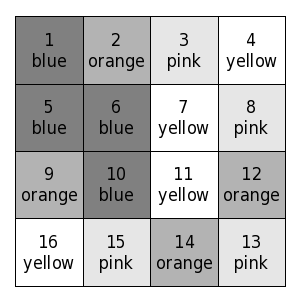
\includegraphics[width=0.4\textwidth]{drawers}
\caption{A schematic view of the filing cabinets.\todo{needs nicer pic}}\label{fig:drawers}
\end{figure}


As described above \todo{needs to be described}, Dale and Reiter's
Incremental Algorithm is a special case of our algorithm, where no
roles are used and a specific order is imposed on the predicates. We
replicated Viethen and Dale's experiment, which tested the Incremental
Algorithm on the drawer domain with all possible preference ordering
given the four predicates
\textsf{color, column, row}, and \textsf{corner}
\cite{viethen06:_algor_for_gener_refer_expres}.  Unsurprisingly, we
get the same results as they did: 98 of the 103 non-relational
descriptions produced by humans can be generated using one of the 24
possible preference orderings.

\newcite{viethen06:_algor_for_gener_refer_expres} also tested Dale and
Haddock's \shortcite{dale91:_gener_refer_expres_invol_relat}
Relational Algorithm on the drawer domain. Surprisingly, it could not
generate \textit{any} of the descriptions produced by humans. To
evaluate our algorithm's use of relations, we tested it on a
representation of the domain using the predicates \textsf{color} and
\textsf{corner} and the roles \textsf{above, below, next to, left of},
and \textsf{right of}. We did not include the \textsf{column} and
\textsf{row} predicates because every drawer can be uniquely
identified through those predicates. Since our algorithm has to
consider predicates before relations, this would mean that no relation
ever gets used. Like for the Incremental Algorithm, we tested all
possible orderings of predicates and roles (with the restriction that
all predicates come before all roles). Our algorithm generates 10 of
the 15 relational descriptions. Of the five that it could not
generate, two mentioned column information, which we excluded from our
domain, and three (which interestingly were all produced by the same
person) are of the format \textit{the blue/pink/yellow/orange drawer
above/below/next to/right of/left of the two blue/pink/yellow/orange
drawers}. This would correspond to the following output from our
algorithm: $C_1 \& \exists R . (C_2 \& \exists R . C_2)$ (where $C_i$
are color predicates and $R$ a role). While our algorithm does not
generate descriptions that contain the same relation on two levels of
embedding for these drawers, it does generate some other, simpler
descriptions for them; for example, $\textsf{orange} \& \exists
\textsf{left\_of} . (\textsf{pink}
\& \textsf{corner})$ which could be rendered as
\textit{the orange drawer left of the pink one in the corner}, or
$\textsf{orange} \& \exists \textsf{below} . \textsf{yellow}$,
which could be rendered as \textit{the orange drawer below the yellow
drawer}.

\todo{should we show some more examples? - ak}




\subsection{Efficiency}

Both the \el\ and the \alc\ algorithms took about 15 milliseconds to
compute distinguishing concepts for all 16 individuals in the Viethen
\& Dale dataset.\footnote{We measured all runtimes on a MacBook Pro
  (Intel Core 2 Duo, 2.16 GHz) running Java 1.6 beta, and allowed the
  Java VM to warm up, i.e.\ just-in-time compile all bytecode, before
  taking the measurements.}

\begin{figure}
  \centering
  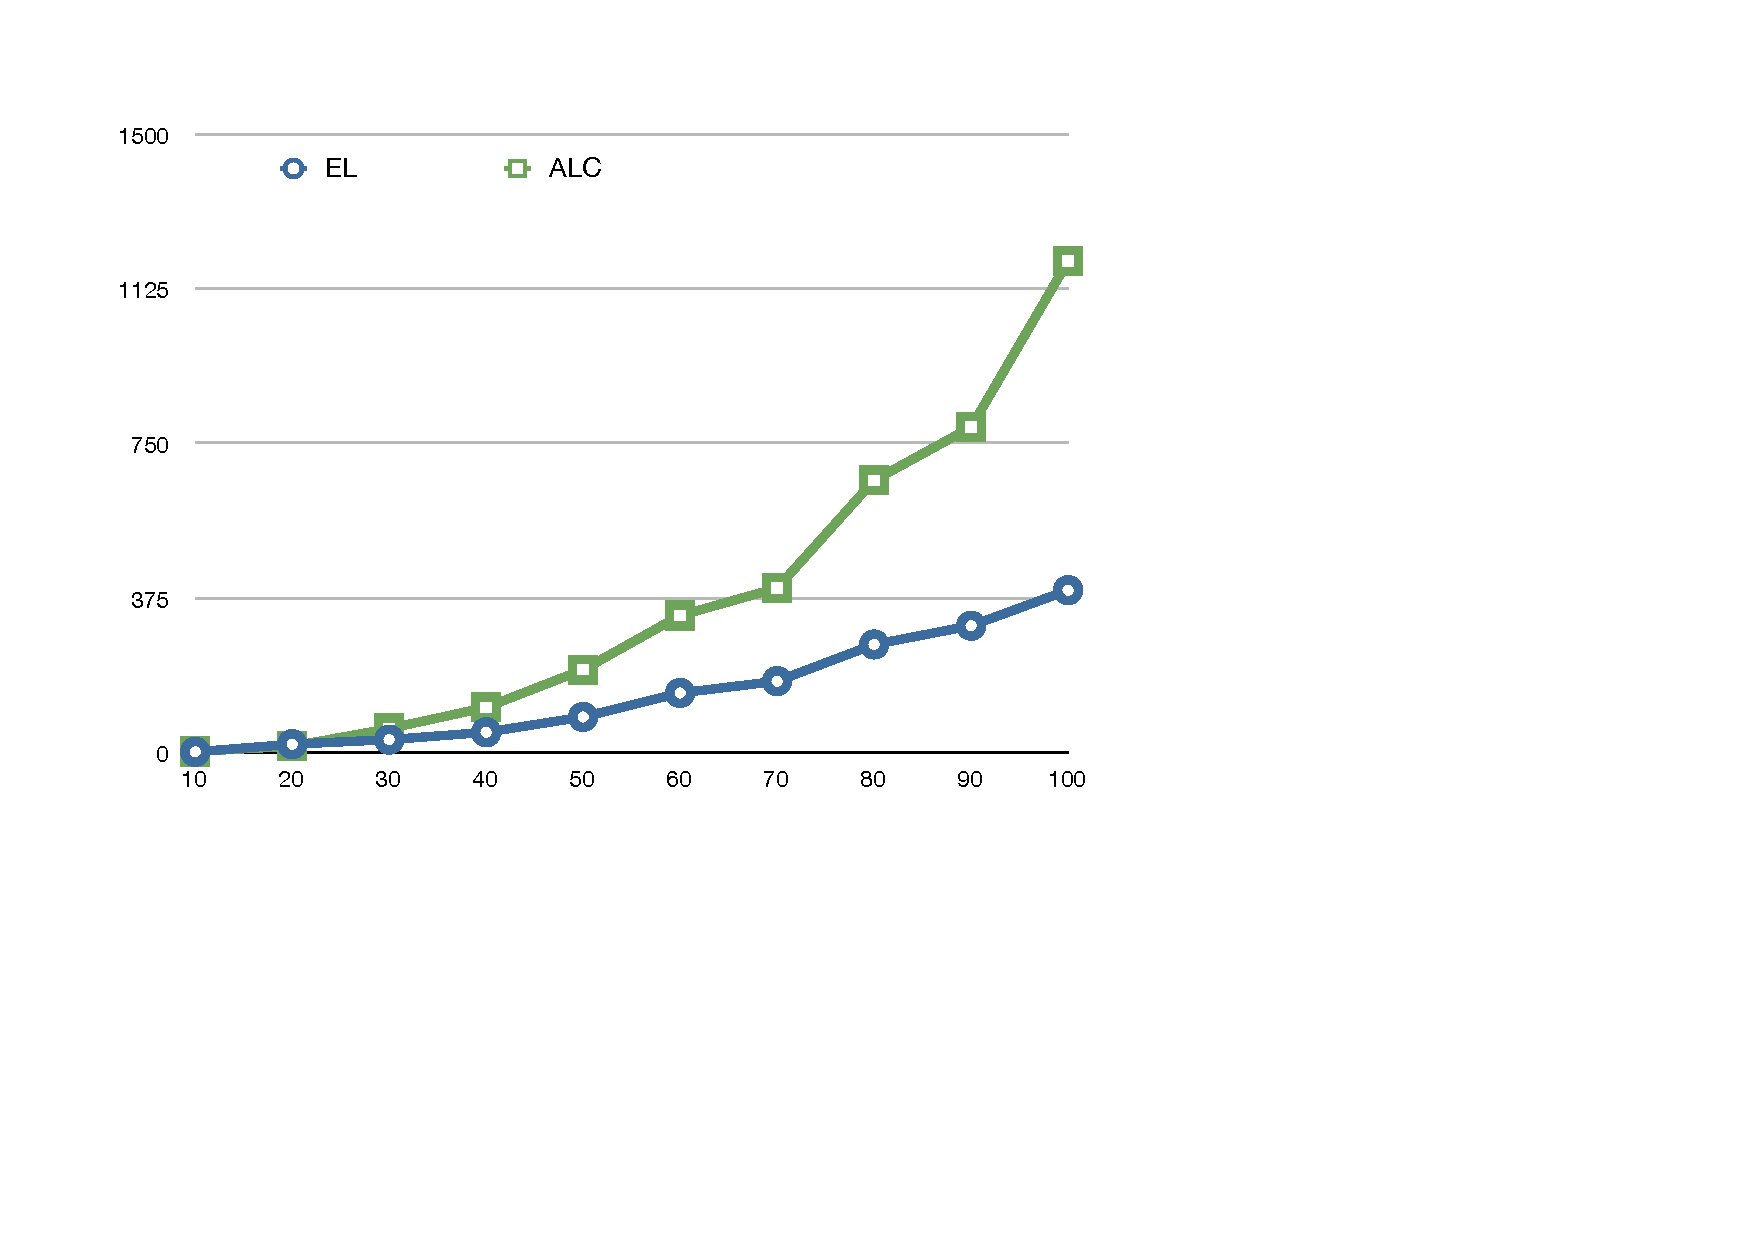
\includegraphics[width=\columnwidth]{runtimes}
  \caption{Average runtimes (in ms) of the two algorithms on random graphs of
    different sizes.} 
  \label{fig:runtimes}
\end{figure}

In order to get a more comprehensive picture of our system's
efficiency, we ran the two algorithms on random graphs with increasing
numbers of nodes.  \todo{harmonize this with what Carlos calls them in
  Section~\ref{sec:bisim}} Each graph had ten different atoms and four
different roles, a 10\% chance for a node to have each atom, and a
10\% chance for each pair of nodes to be connected by each role.  The
results (averaged over 10 runs for each graph size) are shown in
Fig.~\ref{fig:runtimes}.  As the figure shows, the \el\ algorithm
takes about 350 ms on average to generate relational REs for all
individuals in the graph with 100 nodes, i.e.\ 4 ms on average for
each individual.  The \alc\ algorithm is even faster, at about 200 ms
for the graph with 100 nodes.  In both cases, we conclude that the
systems are fast enough for practical use.



\subsection{Interface to realization}

\begin{itemize}
\item there's a risk to generate a concept that can't be realized,
  especially for the \alc\ algorithm
\item everybody except perhaps SPUD has this problem
\item problem is worse in our case because it is harder to control the
  order in which atoms and relations are explored
\item would be interesting for future work to think about how
  search in the bisim algorithms can be controlled by the realizer
\end{itemize}

%%% Local Variables: 
%%% mode: latex
%%% TeX-master: "dl-gre-08"
%%% End: 
